\documentclass[a4paper,12pt]{report}
\usepackage{amssymb}

\usepackage{ucs}
\usepackage[utf8x]{inputenc} % Input encoding for Greek characters
\usepackage[greek,english]{babel} % Language support

\newcommand{\en}{\selectlanguage{english}}
\newcommand{\gr}{\selectlanguage{greek}}

% \usepackage{algorithm2e}
% \usepackage{algorithm}
% \usepackage{algorithmic}
\usepackage{enumitem}
\usepackage{tcolorbox}
\tcbuselibrary{listingsutf8}
\usepackage{float}
\usepackage{amsmath}
\usepackage{graphicx} % For including images
\usepackage{titlesec} % Custom title formatting
\usepackage{fancyhdr} % For custom headers and footers
\usepackage{geometry} % For adjusting page margins

% Adjust the page margins to make content wider
\geometry{top=2.5cm, bottom=2.5cm, left=2.5cm, right=2.5cm}

% Redefine chapter formatting to make it smaller
\titleformat{\chapter}[display]
    {\normalfont\LARGE\bfseries} % Smaller size and bold for chapter heading
    {\chaptername\ \thechapter} % Chapter number format
    {15pt} % Space between chapter number and title
    {\bfseries} % Smaller size and bold for chapter title
\begin{document}

\begin{titlepage}
    \centering
    \vspace*{-3cm}
    % University logo
    \includegraphics[width=1\textwidth]{auth_logo.png} % Replace with your actual logo file

    % University name in Greek
    \textbf{\gr ΑΡΙΣΤΟΤΕΛΕΙΟ ΠΑΝΕΠΙΣΤΗΜΙΟ ΘΕΣΣΑΛΟΝΙΚΗΣ}
    \vspace{2cm}

    % Document title and subtitle in Greek
    \LARGE\textbf{\gr Γραφική με Υπολογιστές Αναφορά} \\
    \Large\normalfont{\gr Εργασία 2} \\
    \vspace{4cm}

    \gr
    \large
    \textbf{Διακολουκάς Δημήτριος} \\
    \textbf{AEM 10642}
    \vspace{2.5cm}

    \en
    \textit{Email: ddiakolou@ece.auth.gr}
\end{titlepage}

\gr
\tableofcontents

\chapter{Περιγραφή Προβλήματος και Ζητούμενα}

\section{Εισαγωγή}

Η δεύτερη εργασία της σειράς μαθημάτων Γραφική με Υπολογιστές εστιάζει στη δημιουργία ενός πλήρους \en pipeline \gr προβολής \en 3D \gr αντικειμένων μέσω μετασχηματισμών, προοπτικής προβολής και τελικής απόδοσης με χρήση υφής (\en texture mapping\gr). Στόχος είναι η κατανόηση της λειτουργίας μίας εικονικής κάμερας, καθώς και η προσομοίωση της κίνησης σε δυναμικά περιβάλλοντα.

\vspace{0.3cm}

\hspace{-0.6cm}Το προς απόδοση αντικείμενο είναι μια \en 3D \gr πυραμίδα, η οποία κινείται πάνω σε κυκλική τροχιά. Η κάμερα μπορεί είτε να είναι σταθερή είτε να ακολουθεί δυναμικά το όχημα \en (camera-follow mode)\gr. Το τελικό αποτέλεσμα είναι δύο animation διάρκειας $5$ δευτερολέπτων το καθένα, που αποθηκεύονται σε μορφή video.

\section{Δοσμένα Δεδομένα – \en hw2.npy \gr και εικόνα}

Το αρχείο \en \texttt{hw2.npy} \gr περιέχει όλα τα απαραίτητα δεδομένα της σκηνής:

\begin{itemize}
    \item \en \textbf{v\_pos:} \gr $3 \times N$ πίνακας με τις τρισδιάστατες συντεταγμένες των κορυφών του αντικειμένου.
    \item \en \textbf{v\_uvs:} \gr $N \times 2$ πίνακας με τις συντεταγμένες υφής \en (UV\gr) για κάθε κορυφή.
    \item \en \textbf{t\_pos\_idx:} \gr $F \times 3$ πίνακας που καθορίζει τα τρίγωνα μέσω δεικτών σε \en \texttt{v\_pos}\gr.
    \item \en \textbf{stone-72\_diffuse.jpg:} \gr Η εικόνα υφής που προβάλλεται στην επιφάνεια του αντικειμένου μέσω \en UV mapping\gr που αναπαριστά έναν βράχο.
    
    \item \en \textbf{k\_road\_center:} \gr Τρισδιάστατο διάνυσμα που δηλώνει το κέντρο της κυκλικής τροχιάς του αυτοκινήτου.
    \item \en \textbf{k\_road\_radius:} \gr Ακτίνα της κυκλικής τροχιάς (τύπου \en \texttt{float}\gr).
    \item \en \textbf{car\_velocitdy:} \gr Ταχύτητα του οχήματος σε μονάδες χώρου ανά δευτερόλεπτο.
    
    \item \en \textbf{k\_cam\_car\_rel\_pos:} \gr Τρισδιάστατο διάνυσμα που καθορίζει τη σχετική θέση της κάμερας ως προς το όχημα.
    \item \en \textbf{k\_cam\_up:} \gr Κανονικοποιημένο διάνυσμα $3 \times 1$ που δηλώνει τον κάθετο προσανατολισμό της κάμερας \en (up vector)\gr.
    \item \en \textbf{k\_cam\_target:} \gr Τρισδιάστατο σημείο-στόχος προς το οποίο κοιτάει η κάμερα (μόνο για \en demo 2\gr).
    
    \item \en \textbf{k\_sensor\_height, k\_sensor\_width:} \gr Διαστάσεις του αισθητήρα της κάμερας σε μονάδες χώρου.
    \item \en \textbf{k\_f:} \gr Εστιακή απόσταση (\en focal length\gr) του μοντέλου κάμερας (τύπου \en \texttt{int}\gr).
    
    \item \en \textbf{k\_duration:} \gr Συνολική διάρκεια προσομοίωσης (σε δευτερόλεπτα).
    \item \en \textbf{k\_fps:} \gr Ρυθμός \en (frames per second) \gr της προσομοίωσης.
\end{itemize}

\section{Ζητούμενα}

Η εργασία ζητά την υλοποίηση των εξής συναρτήσεων:

\begin{enumerate}
    \item \en \textbf{\texttt{translate(t\_vec):}} \gr Δημιουργεί \en affine \gr πίνακα μετατόπισης $4 \times 4$.
    
    \item \en \textbf{\texttt{rotate(axis, angle, center):}} \gr Δημιουργεί \en affine \gr πίνακα περιστροφής $4 \times 4$ γύρω από τυχαίο άξονα.
    
    \item \en \textbf{\texttt{compose(mat1, mat2):}} \gr Σύνθεση δύο \en affine \gr πινάκων μετασχηματισμού.

    \item \en \textbf{\texttt{world2view(pts, R, c0):}} \gr Μετασχηματίζει σημεία από τον παγκόσμιο χώρο \en (WCS) \gr στο σύστημα συντεταγμένων της κάμερας.

    \item \en \textbf{\texttt{lookat(eye, up, target):}} \gr Υπολογίζει τον πίνακα περιστροφής και μετατόπισης της κάμερας ώστε να κοιτά το στόχο.

    \item \en \textbf{\texttt{perspective\_project(pts, focal, R, t):}} \gr Προοπτική προβολή σημείων από \en 3D \gr σε \en 2D \gr επίπεδο, με χρήση \en pinhole \gr μοντέλου κάμερας.

    \item \en \textbf{\texttt{rasterize(pts\_2d, plane\_w, plane\_h, res\_w, res\_h):}} \gr Χαρτογραφεί τις συντεταγμένες από το επίπεδο της κάμερας σε \en pixel \gr συντεταγμένες εικόνας.

    \item \en \textbf{\texttt{render\_object(...):}} \gr Συνδυάζει όλες τις παραπάνω λειτουργίες και επιστρέφει εικόνα της σκηνής με χρήση \en texture shading\gr.
\end{enumerate}

\section{Προσομοιώσεις και Απαιτήσεις}

Θα πρέπει να παραχθούν δύο προσομοιώσεις:

\begin{itemize}
    \item \en \textbf{Demo 1:} \gr Κάμερα στατική ως προς το όχημα, προσανατολισμένη πάντα προς την κατεύθυνση κίνησης. \gr Το διάνυσμα $\hat{z}_c$ είναι πάντα παράλληλο με το διάνυσμα ταχύτητας του αυτοκινήτου.
    \item \en \textbf{Demo 2:} \gr Κάμερα που περιστρέφεται για να κοιτά πάντα ένα σταθερό σημείο \en (\texttt{k\_cam\_target})\gr.
\end{itemize}

\hspace{-0.6cm}Κάθε προσομοίωση πρέπει να διαρκεί $5$ δευτερόλεπτα, με $25$ \en frames \gr ανά δευτερόλεπτο, και να αποθηκεύεται ως αρχείο βίντεο τύπου \en \texttt{.mp4}\gr.

\section{Συναρτήσεις Υλοποίησης Χρωματισμού και Υφής}

Στην παρούσα εργασία, γίνεται χρήση και επαναχρησιμοποίηση βοηθητικών συναρτήσεων από την προηγούμενη εργασία για την υλοποίηση χαρτογράφησης υφής \en (texture mapping) \gr στο νέο \en pipeline \gr της \en \texttt{render\_object}\gr. Οι συναρτήσεις αυτές είναι οι \en \texttt{vector\_interp}\gr, \en \texttt{t\_shading} \gr και \en \texttt{render\_img}\gr.

\subsection*{Συνάρτηση γραμμικής παρεμβολής μεταξύ διανυσμάτων}

Η \en \texttt{vector\_interp(p1, p2, V1, V2, coord, dim)} \gr συνάρτηση αυτή υλοποιεί γραμμική παρεμβολή μεταξύ δύο διανυσμάτων $V_1$, $V_2$ που αντιστοιχούν σε δύο σημεία $p_1$ και $p_2$. Δεχόμενη μια ενδιάμεση τιμή \en \texttt{coord} \gr ως προς τη διάσταση \en \texttt{dim} \gr ($x$ ή $y$), επιστρέφει την παρεμβολημένη τιμή $V$ στο ενδιάμεσο σημείο.

\begin{itemize}
    \item Αν $p_1[idx] = p_2[idx]$, επιστρέφει το $V_1$.
    \item Διαφορετικά, υπολογίζει τον παράγοντα παρεμβολής $t = \frac{coord - p_1}{p_2 - p_1}$.
    \item Επιστρέφει $V = (1 - t) \cdot V_1 + t \cdot V_2$.
\end{itemize}

\vspace{0.3cm}

\subsection*{Συνάρτηση σκίασης υφής}

Η \en \texttt{t\_shading(img, vertices, uv, textImg)} \gr είναι η βασική συνάρτηση απόδοσης υφής \en (texture shading) \gr για κάθε τρίγωνο:

\begin{itemize}
    \item Ταξινομεί τις κορυφές ως προς το $y$ \en (scanline order)\gr.
    \item Για κάθε γραμμή $y$ \en (scanline)\gr, υπολογίζει τα σημεία τομής $A$, $B$ των πλευρών του τριγώνου με την γραμμή.
    \item Παρεμβάλει τα αντίστοιχα $UV$ των $A$, $B$ χρησιμοποιώντας τη \en \texttt{vector\_interp}\gr.
    \item Για κάθε $x$ στο διάστημα $[A_x, B_x]$, παρεμβάλει $UV$ και δειγματοληπτεί το χρώμα από την εικόνα υφής.
    \item Αποθηκεύει το τελικό χρώμα στην εικόνα εξόδου.
\end{itemize}

\hspace{-0.6cm}Η συνάρτηση αυτή είναι απαραίτητη για τον χρωματισμό με βάση την εικόνα υφής και εξασφαλίζει ομαλή παρεμβολή κατά μήκος των ακμών και \en scanlines\gr.

\vspace{0.4cm}

\subsection*{Συνάρτηση απόδοσης εικόνας}

Η \en \texttt{render\_img(faces, vertices, vcolors, uvs, depth, shading, texImg)} \gr είναι η κεντρική ρουτίνα που αναλαμβάνει να ταξινομήσει τα τρίγωνα και να καλέσει τη σωστή τεχνική χρωματισμού για κάθε ένα:

\begin{itemize}
    \item Δέχεται ως είσοδο όλα τα δεδομένα: κορυφές, χρώματα, $UV$, βάθη, συνδεσιμότητα και τύπο \en shading\gr.
    \item Υπολογίζει το μέσο βάθος για κάθε τρίγωνο και τα ταξινομεί κατά φθίνουσα σειρά βάθους.
    \item Για κάθε τρίγωνο:
        \begin{itemize}
            \item Αν \en \texttt{shading = "t"}\gr, καλεί τη \en \texttt{t\_shading}\gr, όπως άλλωστε ενδείκνυται να χρησιμοποιηθεί από την εκφώνηση και στην βασική συνάρτηση \en render\_object(...)\gr.
            \item (σε άλλο σενάριο, θα μπορούσε να καλέσει \en \texttt{f\_shading})\gr.
        \end{itemize}
    \item Επιστρέφει την τελική εικόνα με όλα τα τρίγωνα αποδοσμένα.
\end{itemize}

\vspace{0.3cm}

\hspace{-0.6cm}Η δομή αυτών των συναρτήσεων διατηρεί την αρχιτεκτονική που υλοποιήθηκε στην προηγούμενη εργασία και επιτρέπει την ευκολία σύνδεσης της \en \texttt{render\_img()} \gr με νέα \en pipelines \gr απόδοσης όπως η \en \texttt{render\_object()} \gr της παρούσας εργασίας.


\chapter{Ανάλυση Υλοποίησης Συναρτήσεων Μετασχηματισμών}

\section{Περίληψη Σκοπού}

Οι συναρτήσεις μετασχηματισμών της παρούσας εργασίας στοχεύουν στην υλοποίηση βασικών γραμμικών μετασχηματισμών στο ομογενές σύστημα συντεταγμένων. Ειδικότερα, παρέχονται υλοποιήσεις για μεταφορά \en (translation)\gr, περιστροφή \en (rotation) \gr και σύνθεση μετασχηματισμών \en (composition\gr). Όλες επιστρέφουν \texttt{4×4} πίνακες που χρησιμοποιούνται για την αναπαράσταση και συνδυασμό μετασχηματισμών σε \en 3D \gr γραφικά.

\section{Συνάρτηση \en \texttt{translate()\gr}}

Η συνάρτηση \en \texttt{translate()} \gr δέχεται ένα διάνυσμα μετατόπισης $t \in \mathbb{R}^3$ και επιστρέφει τον αντίστοιχο \en affine \gr μετασχηματισμό σε μορφή πίνακα $4\times4$.

\begin{tcolorbox}[colback=gray!5!white, colframe=black!75!black, title=\en Pseudo-code \gr για \en \texttt{translate}\gr]
\en 
\begin{verbatim}
function translate(t_vec):
    xform = identity_matrix(4)
    xform[:3, 3] = t_vec
    return xform
\end{verbatim}
\gr
\end{tcolorbox}

\noindent Ο πίνακας που επιστρέφεται έχει τη μορφή:
\[
T = 
\begin{bmatrix}
1 & 0 & 0 & t_x \\
0 & 1 & 0 & t_y \\
0 & 0 & 1 & t_z \\
0 & 0 & 0 & 1 \\
\end{bmatrix}
\]

\section{Συνάρτηση \en \texttt{rotate()}\gr}

Η συνάρτηση \en \texttt{rotate()} \gr παράγει τον \en affine \gr μετασχηματισμό περιστροφής ως προς άξονα $a \in \mathbb{R}^3$, γωνία $\theta$ και σημείο $c \in \mathbb{R}^3$.

\begin{tcolorbox}[colback=gray!5!white, colframe=black!75!black, title=\en Pseudo-code \gr για \en \texttt{rotate}\gr]
\en
\begin{verbatim}
function rotate(axis, angle, center):
    normalize(axis)
    R = Rodrigues(axis, angle)
    t = center - R @ center
    xform = identity_matrix(4)
    xform[:3, :3] = R
    xform[:3, 3] = t
    return xform
\end{verbatim}
\gr
\end{tcolorbox}

\hspace{-0.6cm}Η περιστροφή βασίζεται στον αλγόριθμο του \en Rodrigues \gr και μετατοπίζει το κέντρο ώστε να διατηρηθεί η περιστροφή ως προς το σημείο $c$.

\section{Συνάρτηση \en \texttt{compose()}\gr}

Η \en \texttt{compose()} \gr υλοποιεί τον συνδυασμό δύο μετασχηματισμών μέσω πολλαπλασιασμού πινάκων:
\en 
\[
T_{\text{total}} = T_2 \cdot T_1
\]
\gr

\begin{tcolorbox}[colback=gray!5!white, colframe=black!75!black, title=\en Pseudo-code \gr για \en \texttt{compose}\gr]
\en
\begin{verbatim}
function compose(mat1, mat2):
    return mat2 @ mat1
\end{verbatim}
\gr
\end{tcolorbox}

\noindent Αυτή η συνάρτηση είναι ιδιαίτερα χρήσιμη για την εφαρμογή ακολουθιών μετασχηματισμών σε αντικείμενα \en 3D\gr.

\section{Παρατηρήσεις και Συμπεράσματα}

Οι παραπάνω συναρτήσεις συγκροτούν τη βάση για τον καθορισμό της θέσης και του προσανατολισμού των αντικειμένων στον \en 3D \gr χώρο. Ιδιαίτερη προσοχή δίνεται στην κανονικοποίηση των διανυσμάτων και τη διατήρηση των \en affine \gr ιδιοτήτων. Η υλοποίηση είναι πλήρως συμβατή με το \en pipeline \gr του \en \texttt{render\_object} \gr της εργασίας.

\chapter{Υλοποίηση βασικών συναρτήσεων}

Σε αυτό το κεφάλαιο αναλύονται οι βασικές συναρτήσεις που χρησιμοποιούνται για τον υπολογισμό των μετασχηματισμών προβολής και την απόδοση του τελικού αντικειμένου στην εικόνα. Οι συναρτήσεις αυτές περιλαμβάνουν μετατροπή συντεταγμένων, ορισμό συστήματος κάμερας, προβολή και \en rasterization\gr.

\section{Μετατροπή Συντεταγμένων: \en \texttt{world2view()}\gr}

Η συνάρτηση \en \texttt{world2view} \gr μετατρέπει τις συντεταγμένες ενός σημείου από το παγκόσμιο σύστημα αναφοράς στο σύστημα της κάμερας. Ο τύπος που χρησιμοποιείται είναι:

\en
\[
p_{\text{view}} = R \cdot (p_{\text{world}} - c_0)
\]
\gr

\noindent όπου $R$ είναι ο πίνακας περιστροφής της κάμερας και $c_0$ είναι η θέση της.

\begin{tcolorbox}[colback=gray!5!white, title=\en Pseudo-code \texttt{world2view}\gr]
\en
\begin{verbatim}
function world2view(pts, R, c0):
    for each point p in pts:
        p_view = R @ (p - c0)
    return all transformed points as Nx3
\end{verbatim}
\gr
\end{tcolorbox}

\section{Ορισμός Συστήματος Κάμερας: \en \texttt{lookat()}\gr}

Η \en \texttt{lookat} \gr δημιουργεί το σύστημα συντεταγμένων της κάμερας με βάση τη θέση της κάμερας \en \texttt{eye}\gr, το σημείο στόχο \en \texttt{target} \gr και το διάνυσμα προς τα πάνω \en \texttt{up}\gr. Η περιστροφή $R$ δημιουργείται από τρεις ορθογώνιους άξονες:

\[
\hat{z}_c = \frac{target - eye}{\|target - eye\|}, \quad
\hat{x}_c = \frac{\hat{z}_c \times up}{\|\hat{z}_c \times up\|}, \quad
\hat{y}_c = \hat{x}_c \times \hat{z}_c
\]

\begin{tcolorbox}[colback=gray!5!white, title=\en Pseudo-code  \texttt{lookat}\gr]
\en
\begin{verbatim}
function lookat(eye, up, target):
    z = normalize(target - eye)
    x = normalize(cross(z, up))
    y = cross(x, z)
    return [x, y, -z] as rotation matrix R, and eye as translation
\end{verbatim}
\gr
\end{tcolorbox}

\section{Προοπτική Προβολής: \en \texttt{perspective\_project()}\gr}

Η συνάρτηση \en \texttt{perspective\_project} \gr μετασχηματίζει τα σημεία από \en 3D \gr σε \en 2D \gr με χρήση του εστιακού μήκους $f$, εφαρμόζοντας την προοπτική προβολή:

\[
x' = \frac{f}{z} \cdot x, \quad y' = \frac{f}{z} \cdot y
\]

\noindent και διατηρεί το βάθος κάθε σημείου.

\begin{tcolorbox}[colback=gray!5!white, title=\en Pseudo-code \texttt{perspective\_project}\gr]
\en
\begin{verbatim}
function perspective_project(pts, focal, R, t):
    pts_view = world2view(pts, R, t)
    for each point p:
        x' = (focal / p.z) * p.x
        y' = (focal / p.z) * p.y
    return [x', y'] and depth
\end{verbatim}
\gr
\end{tcolorbox}

\section{Μετατροπή σε Εικονοστοιχεία: \en \texttt{rasterize()}\gr}

Η \en \texttt{rasterize} \gr μετατρέπει τις κανονικοποιημένες \en 2D \gr συντεταγμένες σε θέσεις εικονοστοιχείων, με βάση τις διαστάσεις του καμβά και του αισθητήρα. Οι τελικές τιμές περιορίζονται στα όρια της εικόνας.

\begin{tcolorbox}[colback=gray!5!white, title=\en Pseudo-code  \texttt{rasterize}\gr]
\en
\begin{verbatim}
function rasterize(pts_2d, plane_w, plane_h, res_w, res_h):
    for each point (x, y):
        pixel_x = x * scale_x + center_x
        pixel_y = -y * scale_y + center_y
        clamp to [0, res-1]
    return pixel coordinates
\end{verbatim}
\gr
\end{tcolorbox}

\section{Απόδοση Αντικειμένου: \en \texttt{render\_object()}\gr}

Η βασική συνάρτηση \en \texttt{render\_object} \gr συνδυάζει όλα τα παραπάνω βήματα για την τελική απόδοση του \en 3D \gr μοντέλου στην εικόνα:

\begin{itemize}
    \item Υπολογίζει τον μετασχηματισμό κάμερας \en (\texttt{lookat})\gr
    \item Εφαρμόζει την προβολή \en (\texttt{perspective\_project})\gr
    \item Μετατρέπει σε \en pixels (\texttt{rasterize})\gr
    \item Επιστρέφει τελική εικόνα με χρήση \en \texttt{render\_img}\gr
\end{itemize}

\begin{tcolorbox}[colback=gray!5!white, title=\en Pseudo-code \texttt{render\_object}\gr]
\en
\begin{verbatim}
function render_object(...):
    R, t = lookat(eye, up, target)
    pts_2d, depth = perspective_project(v_pos, focal, R, t)
    pixel_coords = rasterize(pts_2d, plane_w, plane_h, res_w, res_h)
    vertices = concat(pixel_coords, depth)
    image = render_img(faces,vertices,vcolors,uvs,depth,"t",texImg)
    return image
\end{verbatim}
\gr
\end{tcolorbox}

\hspace{-0.6cm}Όλες οι παραπάνω συναρτήσεις έχουν υλοποιηθεί εντός του αρχείου \en all\_functs.py \gr

\chapter{Ανάλυση αποτελεσμάτων, συμπεράσματα και οπτικοποίηση}

Σε αυτό το κεφάλαιο παρουσιάζεται η ανάλυση των εκτελέσιμων αρχείων \en \texttt{demo1.py} \gr και \en \texttt{demo2.py}\gr, τα οποία παράγουν δυναμικές προσομοιώσεις βασισμένες στις συναρτήσεις που υλοποιήθηκαν στα προηγούμενα κεφάλαια. Η ανάλυση επικεντρώνεται στη ροή των συναρτήσεων, στη δομή των αρχείων και στην τελική παραγωγή καρέ και βίντεο.

\section{Αρχείο \en \texttt{demo1.py} \gr -- Προσομοίωση με \en Forward Facing Camera\gr}

Το αρχείο \en \texttt{demo1.py} \gr (συγκεκριμένα η \en \texttt{render\_forward\_demo(...)}\gr) υλοποιεί την περίπτωση όπου η κάμερα είναι σταθερά στραμμένη προς την κατεύθυνση κίνησης του οχήματος.

\begin{itemize}
    \item Η συνάρτηση \en \texttt{load\_data()} \gr φορτώνει τα απαραίτητα δεδομένα (\en \texttt{hw2.npy}\gr) και την εικόνα υφής.
    
    \item Κάθε καρέ αντιστοιχεί σε χρονική στιγμή $t = \frac{\text{\en frame \gr}}{\text{\en fps \gr}}$.
    
    \item Η γωνιακή θέση του οχήματος υπολογίζεται ως $\theta = \omega t$, όπου $\omega = \frac{v}{r}$ είναι η γωνιακή ταχύτητα.
    
    \item Η θέση του αυτοκινήτου και η θέση της κάμερας προκύπτουν με χρήση ημιτονοειδών συναρτήσεων πάνω σε κυκλική τροχιά.
    
    \item Το διάνυσμα \en \texttt{tangent} \gr υπολογίζεται ως εφαπτόμενο της τροχιάς και χρησιμοποιείται για τον προσδιορισμό του σημείου \en \texttt{target}\gr, δηλαδή του σημείου προς το οποίο κοιτά η κάμερα.
    
    \item Η \en \texttt{render\_object()} \gr λαμβάνει όλα τα παραπάνω και δημιουργεί το καρέ μέσω των εξής συναρτήσεων:
    \begin{itemize}
        \item \en \texttt{lookat()} \gr – Υπολογισμός μετασχηματισμού από παγκόσμιο σε σύστημα κάμερας.
        \item \en \texttt{perspective\_project()} \gr – Προβολή σημείων στον \en 2D \gr καμβά.
        \item \en \texttt{rasterize()} \gr – Αντιστοίχιση προβολών σε \en pixels\gr.
        \item \en \texttt{render\_img()} \gr – Απόδοση χρωμάτων με \en texture shading\gr.
    \end{itemize}

    \item Η εικόνα αποθηκεύεται με \en \texttt{plt.imsave()} \gr και προστίθεται στο βίντεο τύπου \en .mp4 \gr μέσω \en \texttt{imageio.mimsave()}\gr και το βίντεο διαρκεί 5 \en sec \gr στα \en 25 fps\gr.
\end{itemize}

\subsection{Αποτελέσματα \en Farward Facing Camera\gr}
Παρακάτω παρατίθενται ορισμένα αποτελέσματα ανά χρονική στιγμή του βίντεο (αριθμός \en frame\gr) στην περίπτωση της εκτέλεσης στο \en demo1.py \gr.

\begin{figure}[H]
    \centering
    \begin{tabular}{cc}
        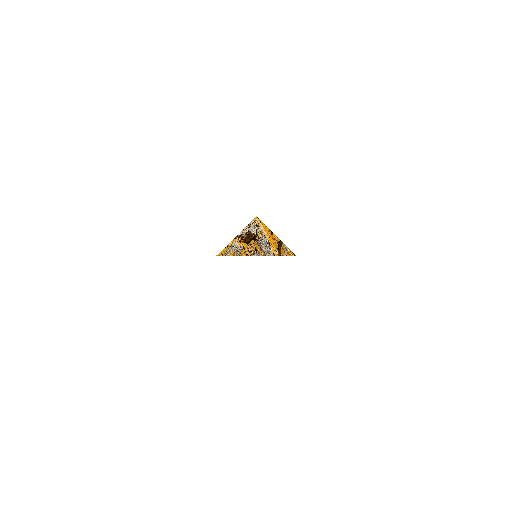
\includegraphics[width=0.45\textwidth]{frame_000.png} &
        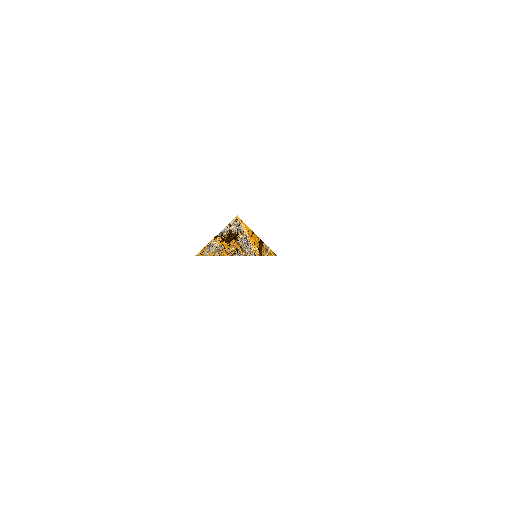
\includegraphics[width=0.45\textwidth]{frame_030.png} \\
        \gr Καρέ 0 από \en \texttt{demo1.py} \gr & \gr Καρέ 30 από \en \texttt{demo1.py} \gr\\
        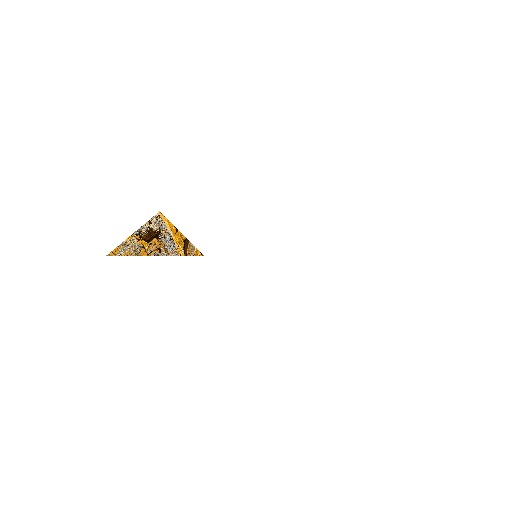
\includegraphics[width=0.45\textwidth]{frame_080.png} &
        
\includegraphics[width=0.45\textwidth]{frame_124.png} \\
        \gr Καρέ 60 από \en \texttt{demo1.py} \gr & \gr Καρέ 90 από \en \texttt{demo1.py} \gr
    \end{tabular}
    \caption{\gr Χαρακτηριστικά καρέ από την εκτέλεση του \en \texttt{demo1.py} \gr καθώς το αντικείμενο κινείται και η κάμερα ακολουθεί τη φορά κίνησης.}
\end{figure}

\hspace{-0.6cm}Εκτελώντας το αρχείο \en \texttt{demo1.py} \gr δημιουργείται ένα βίντεο \en 5s \gr στα \en 25 fps \gr με συνολικά $125$ καρέ, αποθηκευμένο ως \en \texttt{demo\_1\_video.mp4}\gr, ενώ οι εικόνες συλλέγονται σε \en folder \gr που θα δημιουργηθεί ονόματι \en demo\_1\gr.

\section{Αρχείο \en \texttt{demo2.py} \gr -- Προσομοίωση με \en Target Tracking Camera\gr}

Το αρχείο \en \texttt{demo2.py} \gr (και ειδικότερα η \en \texttt{render\_target\_tracking\_demo(...)}\gr) υλοποιεί το σενάριο κατά το οποίο η κάμερα είναι μονίμως προσανατολισμένη σε ένα σταθερό σημείο \en \texttt{target} \gr του χώρου, ανεξάρτητα από την κατεύθυνση της κίνησης του οχήματος.

\begin{itemize}
    \item Όπως και στην προηγούμενη περίπτωση, η \en \texttt{load\_data()} \gr διαβάζει τα δεδομένα γεωμετρίας και την υφή.
    
    \item Η θέση του οχήματος υπολογίζεται μέσω του τύπου:
    \en
    \[
        \theta = \omega t, \quad \omega = \frac{v}{r}
    \]
    \[
        \texttt{car\_pos} = \texttt{center} + r \cdot [\cos(\theta), 0, \sin(\theta)]
    \]
    \gr

    \item Η θέση της κάμερας \en \texttt{cam\_pos} \gr παραμένει ίδια με την περίπτωση του \en \texttt{demo1.py}\gr, όμως ο στόχος \en \texttt{target} \gr είναι προκαθορισμένος από το αρχείο \en \texttt{hw2.npy} \gr και παραμένει σταθερός.

    \item Η συνάρτηση \en \texttt{render\_object()} \gr καλείται με διαφορετικό \en \texttt{target} \gr για κάθε καρέ, ο οποίος δεν σχετίζεται με την κατεύθυνση κίνησης.

    \item Η απεικόνιση γίνεται και εδώ με τη χρήση \en texture mapping\gr, ενώ η διαδικασία αποθήκευσης και δημιουργίας του τελικού βίντεο είναι πανομοιότυπη με την περίπτωση του \en demo1.py\gr.
\end{itemize}

\subsection{Αποτελέσματα \en Target Tracking Camera\gr}

Στην παρακάτω εικόνα παρουσιάζονται τέσσερα καρέ που αντιστοιχούν σε διαφορετικές χρονικές στιγμές της εκτέλεσης του \en \texttt{demo2.py}\gr. Σε κάθε καρέ παρατηρείται ότι η κάμερα ακολουθεί σταθερά το σημείο στόχο, ανεξαρτήτως της κατεύθυνσης κίνησης.

\begin{figure}[H]
    \centering
    \begin{tabular}{cc}
        \includegraphics[width=0.45\textwidth]{frame_000_2.png} &
        \includegraphics[width=0.45\textwidth]{frame_030_2.png} \\
        \gr Καρέ 0 από \en \texttt{demo2.py} \gr & \gr Καρέ 30 από \en \texttt{demo2.py} \gr\\
        \includegraphics[width=0.45\textwidth]{frame_080_2.png} &
        \includegraphics[width=0.45\textwidth]{frame_124_2.png} \\
        \gr Καρέ 80 από \en \texttt{demo2.py} \gr & \gr Καρέ 124 από \en \texttt{demo2.py} \gr
    \end{tabular}
    \caption{\gr Χαρακτηριστικά καρέ από την εκτέλεση του \en \texttt{demo2.py} \gr με την κάμερα προσηλωμένη σε σταθερό \en target point.}
\end{figure}

\hspace{-0.6cm}Εκτελώντας το αρχείο \en \texttt{demo2.py} \gr δημιουργείται ένα βίντεο \en 5s \gr στα \en 25 fps \gr με συνολικά $125$ καρέ, αποθηκευμένο ως \en \texttt{demo\_2\_video.mp4}\gr, ενώ οι εικόνες συλλέγονται σε \en folder \gr που θα δημιουργηθεί ονόματι \en demo\_2\gr.

\section{Συμπεράσματα και Παρατηρήσεις}

Η παρούσα εργασία περιελάμβανε την υλοποίηση δύο διαφορετικών σεναρίων προβολής τρισδιάστατου αντικειμένου σε \en 2D \gr καμβά, μέσα από την προσομοίωση κάμερας που κινείται ή παραμένει σταθερά προσηλωμένη σε ένα σημείο στόχο. Τα αποτελέσματα από τα δύο σενάρια παρουσιάστηκαν παραπάνω.

\begin{itemize}
    \item Στην περίπτωση του \en \texttt{demo1.py} \gr, η κάμερα είναι \textbf{ευθυγραμμισμένη με τη φορά κίνησης του οχήματος}, καθώς το διάνυσμα στόχευσης προκύπτει προσθέτοντας το \en \texttt{tangent} \gr διάνυσμα στη θέση της κάμερας. Αυτό έχει ως αποτέλεσμα το αντικείμενο να αλλάζει θέση και μέγεθος μέσα στο κάδρο. Η κάμερα ακολουθεί την πορεία του οχήματος και παρατηρούμε μια συνεχή αλλαγή οπτικής γωνίας, η οποία προσφέρει μια πιο δυναμική εμπειρία παρατήρησης.

    \item Αντίθετα, στο \en \texttt{demo2.py} \gr, η κάμερα είναι \textbf{σταθερά στραμμένη σε συγκεκριμένο στόχο} (\en target point\gr) καθ’ όλη τη διάρκεια της προσομοίωσης. Το σημείο αυτό παραμένει σταθερό στον χώρο, και η κάμερα περιστρέφεται γύρω του καθώς το όχημα κινείται κυκλικά. Ως αποτέλεσμα, η προοπτική παραμένει σχεδόν σταθερή και το αντικείμενο φαίνεται σχεδόν ακίνητo στο κέντρο της εικόνας, παρότι το όχημα αλλάζει θέση στο χώρο.
    
    \item Και στις δύο περιπτώσεις, η τεχνική \en \texttt{texture shading} \gr λειτουργεί σωστά και αποδίδει με επιτυχία την υφή πάνω στην επιφάνεια του αντικειμένου.
    
    \item Η χρήση της συνάρτησης \en \texttt{lookat()} \gr αποδείχθηκε κομβική για τον ορισμό του συστήματος συντεταγμένων της κάμερας, καθώς και για την ορθή μετατροπή των σημείων από το \en WCS \gr στο σύστημα της κάμερας.
    
    \item Η χρήση διαφορετικών μεθόδων υπολογισμού του \en \texttt{target} \gr οδήγησε σε δύο ενδιαφέρουσες, οπτικά διακριτές προσομοιώσεις, οι οποίες ενισχύουν την κατανόηση της λειτουργίας του πλαισίου απόδοσης εικόνας από τρισδιάστατα μοντέλα.
\end{itemize}

\vspace{0.3cm}

\noindent Συνολικά, η εργασία ανέδειξε τη σημασία του σωστού ορισμού της θέσης και κατεύθυνσης της κάμερας για την παραγωγή δυναμικής ή σταθερής οπτικής προσομοίωσης. Η επιτυχής ενσωμάτωση των συναρτήσεων \en \texttt{lookat, perspective\_project, rasterize, render\_img} \gr και η δημιουργία των βίντεο αποτελούν απόδειξη της σωστής υλοποίησης του συστήματος προβολής και απόδοσης τρισδιάστατων δεδομένων.

\bibliographystyle{plain}
\begin{thebibliography}{1}
    \bibitem{first_bibl}
    \en https://docs.opencv.org/4.x/d9/df8/tutorial\_root.html
    \bibitem{second_bibl}
    \en https://imageio.readthedocs.io/en/stable/
\end{thebibliography}

\end{document}